\subsection{Geometric Interpretation of Tangential Gradients} \label{ssec:3DGradGeometric}
Precise definition and analysis of the Sobolev spaces $\tgradSob{\ddom}{\dddmes}$ can be found in section \ref{sec:BorelMeasSobSpaces}, and explicit analysis of these spaces in section \ref{sec:3DGradSobSpaces}.
Our objective here is to provide the reader with an intuitive idea for the objects $\tgrad_{\ddmes}u$ and $\tgrad_{\dddmes}u$, and provide directs for the interested reader to the relevant analysis.

The intuition behind the form of the tangential gradients (and gradients of zero) with respect to the various measures $\lambda_{jk}, \ddmes, \massMes$, and $\dddmes$ can be summarised with the colloquial phrase ``tangential gradients only reflect behaviour that the measure can see".
Let us be more precise, and first consider the measure $\lambda_{jk}$ for a fixed $I_{jk}$ and the associated gradients of zero and tangential gradients.
Suppose that we have a (sufficiently smooth) function $u$ defined on $\ddom$ that satisfies $u=0$ on $I_{jk}$; from the perspective of $\lambda_{jk}$ this $u$ is the zero function\footnote{More precisely, $u$ is represented by the zero function in $\ltwo{\ddom}{\lambda_{jk}}$.}, regardless of whether $u$ is zero on the whole of $\ddom$ or not.
So despite $u=0$ in $\ltwo{\ddom}{\lambda_{jk}}$, it can have any profile in the direction $n_{jk}$ \emph{as it crosses} $I_{jk}$ and thus any kind of (reasonable) behaviour in the rest of $\ddom$ (propositions \ref{prop:3DGradZeroParallel} and \ref{prop:3DGradZeroRotated}).
In an analogue with classical gradients, the measure $\lambda_{jk}$ is unable to deduce whether (for $x\in I_{jk}$) $u(x+hn_{jk})$ is different from $u(x)$ for $h\neq0$, given the only information it can have about the function $u$ are its values on $I_{jk}$.
Consequentially, the measure $\lambda_{jk}$ cannot bestow a concept of normal derivative $\pdiff{u}{n_{jk}}$ --- changing the profile of $u$ across the edge $I_{jk}$ does not change $u$ on $I_{jk}$.
Conversely, the component of any ``gradient" directed along $n_{jk}$ corresponds to no change in the function $u$ in the eyes of $\lambda_{jk}$.
This is schematically illustrated in figure \ref{fig:Diagram_GradZeroIllustrations}, where along an edge $I_{jk}$ each of the plotted functions are zero, however their behaviour outside $I_{jk}$ is very different.
\begin{figure}[b!]
	\centering
	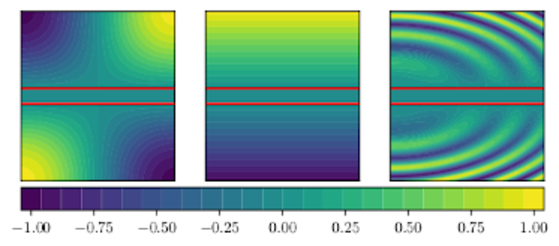
\includegraphics[scale=1.0]{Diagram_GradZeroIllustrations-Scaled.pdf}
	\caption{\label{fig:Diagram_GradZeroIllustrations} Examples illustrating how gradients of zero can arise. The region between the red lines represents an edge $I_{jk}$, which has been thickened to aid in visualisation. Despite each of the plotted functions being constantly zero along the edge $I_{jk}$, and thus equal to the zero function in the eyes of $\lambda_{jk}$, each function is changing in the direction $n_{jk}$ as it crosses $I_{jk}$.}
\end{figure}
A gradient that corresponds to no change in function must be (from our classical understanding) the gradient of a constant, or by our new understanding, a gradient of zero.
Again with an analogue to classical gradients, the measure $\lambda_{jk}$ \emph{does} allows us to evaluate expressions like $u(x+he_{jk})-u(x)$ --- that is, we can detect changes in the function along $I_{jk}$.
Such changes correspond to $u$ changing in the direction tangential to the edge ($\pdiff{u}{e_{jk}}\neq 0$ classically), and thus we find that tangential gradients are directed along $e_{jk}$.
Since our singular measure is just the Lebesgue measure along $I_{jk}$, the tangential gradient is related to the classical (weak) derivative along the interval associated to $I_{jk}$ (proposition \ref{prop:3DTangGradParallel}, corollary \ref{cory:3DTangGradRotated}).
This also highlights the reason for defining the gradients of zero and tangential gradients as in section \ref{sec:BorelMeasSobSpaces} --- given a tangential gradient $\ktgrad_{\lambda_{jk}}u$, $\lambda_{jk}$ can reconstruct the function $u$ along the edge $I_{jk}$, but cannot determine what $u$ is doing across $I_{jk}$.
Ergo, every function has a gradient that is unique up to a gradient of zero, because there is no way for $\lambda_{jk}$ to determine what $u$ looks like across (and thus outside of) $I_{jk}$.

The measure $\ddmes$ is then just a sum of each of the edge measurs $\lambda_{jk}$, so it is not unsurprising for us to find that we can extend gradients of zero on edges $I_{jk}$ by zero to the whole of $\graph$, and conversely the restriction of a gradient of zero to $I_{jk}$ is a gradient of zero with respect to $\lambda_{jk}$ (proposition \ref{prop:3DGradZeroChar}).
Consequentially, the behaviour of tangential gradients with respect to $\ddmes$ on $I_{jk}$ is simply that of the tangential gradient with respect to $\lambda_{jk}$ (theorem \ref{thm:3DTangGradGraph}(i)-(ii)).
However the connectivity of $\graph$ also exerts influence on the functions that possess tangential gradients, and we are also able to deduce that functions that possess tangential gradients are also continuous at each of the vertices $v_j\in\vertSet$ (theorem \ref{thm:3DTangGradGraph}(iii)).
Whilst this can be interpreted as an analogue to the classical situation in which ``a differentiable function is continuous", it is mainly a consequence of our method of constructing tangential gradients through approximating sequences.
We cannot have arbitrarily large ``jumps" at the vertices of our graph, else the gradients of the \emph{smooth} approximating functions will become too large to control in the vicinity of this vertex, and in particular on the connecting edges.

The above story is similar when considering the tangential gradient of $u$ with respect to the measure $\massMes$.
However the ``view" of $\massMes$ is even more restricted than $\lambda_{jk}$, only being able to view the value of $u$ at the vertices, which are a set of isolated points in $\ddom$.
As such, there is no way for the measure $\massMes$ to reconstruct any kind of sensible gradient --- regarding a classical analogoue, there are no ``nearby" function values $u\bracs{v_j + h x}, x\neq 0$ to compare the value of $u\bracs{v_j}$ to.
The result is proposition \ref{prop:NuGradZeroChar}; any gradient must be a gradient of zero because as far as $\massMes$ is concerned, there is no visible change in $u$ in any neighbourhood of $v_j$.
Correspondingly, the tangential gradients are essentially zero everywhere (corollary \ref{cory:NuTangGradChar}).
Then given that $\dddmes$  is just the sum of the measures $\ddmes$ and $\massMes$, we find that $\tgrad_{\dddmes}u$ inherits the behaviours from $\ddmes$ and $\massMes$.
In summary, for a function $u\in\tgradSob{\ddom}{\dddmes}$;
\begin{enumerate}[(a)]
	\item The function $u$ is continuous at all vertices $v_j\in\vertSet$.
	\item On each edge $I_{jk}\in\edgeSet$, $\tgrad_{\dddmes}u = \tgrad_{\lambda_{jk}}u$, and $\tgrad_{\lambda_{jk}}u = \bracs{\bracs{u^{(jk)}}' + \rmi\qm_{jk}u^{(jk)}}e_{jk}$.
	The function $\bracs{u^{(jk)}}'$ being the derivative (in the $H^1$-sense) of the function $u^{(jk)}\circ r_{jk}$.
	\item At each vertex $v_j\in\vertSet$, we have $\tgrad_{\dddmes}u=0$, however $\lim_{x\rightarrow v_j}\tgrad_{\lambda_{jk}}u$ need not be zero.
\end{enumerate}
It is also worth noting that (b) informs us that $\tgrad_{\dddmes}u = \ograd_{\dddmes}u + \rmi\Theta u$, where 
\begin{align*}
	\Theta(x) = 
	\begin{cases} \qm_{jk}e_{jk} & x\in I_{jk}, \\ 0 & x\in\vertSet, \end{cases}
\end{align*}
so all tangential gradients are identical up to a multiple of the quasi-momentum multiplying the original function $u$ on each edge.
This is to be expected from our use of the Gelfand transform; we expect that each of our fibres to act on the same function space through a ``$\qm$-shifted gradient", which they effectively do as shown by the above.
That being said, it was not obvious from the start our of analysis what the shift $\Theta$ should be --- however now we observe that the appropriate ``shift" is to take the component of the quasi-momentum that lies in the direction of each edge, or rather in the direction that the tangential gradient points in.
This is not unexpected given that the gradient has a natural 1D analogue in the derivative, however we do not have such analogies when we come to consider curls or divergences of vector fields.
However, with the analysis of section \ref{sec:3DGradSobSpaces} we are granted a method through which we can identify the ``correct" derivative-like objects to work with.
Furthermore, one can also use this analysis to consider relaxing the restrictions on the embedding of $\graph$ itself, in particular relaxing the requirement that the edges be straight segments --- we discuss this further in section \ref{ssec:CurvedEdges}.